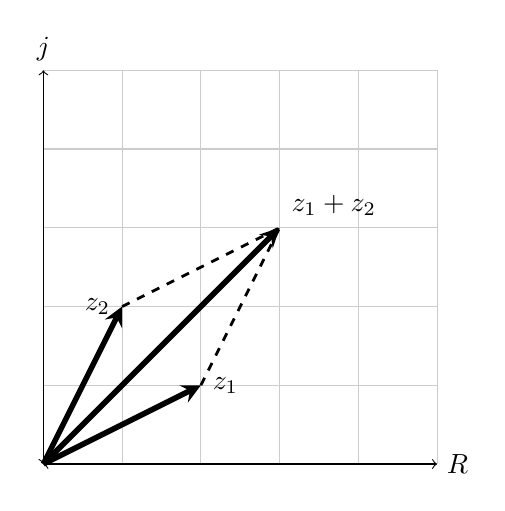
\begin{tikzpicture}
        \draw[thin,gray!40] (0,0) grid (5,5);
        \draw[<->] (0,0)--(5,0) node[right] {$R$};
        \draw[<->] (0,0)--(0,5) node[above]{$j$};
       \draw[line width=2pt,black,-stealth](0,0)--(1,2) node[left]{${z_2}$};
       \draw[line width=2pt,black,-stealth](0,0)--(2,1) node[right]{${z_1}$};
       \draw[line width=2pt,black,-stealth](0,0)--(3,3) node[anchor=south west]{${z_1+z_2}$};
       \draw[line width=1pt,black,dashed](1,2)--(3,3);
       \draw[line width=1pt,black,dashed](2,1)--(3,3);
    \end{tikzpicture}
    \caption{Representacion de la suma entre 2 numeros complejos}